\documentclass{article}
%Seitenränder
\usepackage{geometry}
\geometry{a4paper, left=30mm, right=30mm, top=25mm, bottom=25mm} 

%Encoding:
\usepackage{t1enc}
\usepackage[utf8]{inputenc}

%Mathematische Formeln:
\usepackage{amsmath}
\usepackage{amsfonts}
\usepackage{amssymb}
\usepackage{mathtools} %Erweitert das amsmath package
\usepackage{yhmath} %Erweiterte Schriftarten in Mathe-Umgebungen

\usepackage{graphicx}
\usepackage{framed}
% for \Yleft \Yright
\usepackage{stmaryrd}
\usepackage{xcolor} %Text und Grafiken farbig gestalten
\usepackage{multicol} %Mehrspaltiger Text

\usepackage{hyperref} %Verwandelt u.a. interne links in klickbare Verweise
\usepackage[shortlabels]{enumitem} %itemize, enumerate, description individuell anpassen
\usepackage{float} %Grafiken schöner einfügen
\usepackage{wrapfig} %Von Text umflossene Grafiken einfügen
\usepackage{tikz} %Automaten, Graphen, ... mit LaTeX darstellen
\usetikzlibrary{arrows,shapes,automata,petri,backgrounds,calc,intersections}

\usepackage{todonotes}
\usepackage[toc]{appendix}


% Titel in Kopfzeilen
\usepackage{fancyhdr}
\pagestyle{fancy}
\setlength{\headheight}{20pt}


% Format der Autorenkürzel definieren
\newcommand{\initials}[1]{\small{\textit{(#1)}} \normalsize}

%----------------------------------------------
% Hier euren Titel eintragen
\title{Implementing a CSP Solver\\\small{Lecture Hybrid Systems, summer '19}}
% Hier eure(n) Namen eintragen
\author{Patrick Burke and Lynn Liebert}

%Kopfzeile anpassen:
\fancyhead[R]{CSP Solver} %Hier Dokument-Titel eintragen (erscheint im Header). Falls eigentlicher Titel zu lang, hier Kurztitel einfügen!
\fancyhead[L]{P. Burke, L. Liebert} %Auch hier ggf. Kurzversionen der Namen, falls Header zu voll wird.

%Damit werden euer Titel und der Autor intern definiert (hier müsst ihr nichts ändern)
\hypersetup{
	pdftitle={\@title},
	pdfauthor={\@author}
}


\newtheorem{theorem}{Theorem}[section]
\newtheorem{corollary}{Corollary}[theorem]
\newtheorem{lemma}[theorem]{Lemma}

\DeclareRobustCommand\full  {\tikz[baseline=-0.6ex]\draw[thick] (0,0)--(0.5,0);}
\DeclareRobustCommand\dotted{\tikz[baseline=-0.6ex]\draw[thick,dotted] (0,0)--(0.54,0);}
\DeclareRobustCommand\dashed{\tikz[baseline=-0.6ex]\draw[thick,dashed] (0,0)--(0.54,0);}
\DeclareRobustCommand\chain {\tikz[baseline=-0.6ex]\draw[thick,dash dot dot] (0,0)--(0.5,0);}

%Beginn des eigentlichen Dokumentes:
%----------------------------------------------
\begin{document}
\maketitle %Setzt automatisch Titel, Autoren und Datum

\listoftodos

\begin{abstract}
\todo[inline]{ABSTRACT}
\end{abstract}

\tableofcontents
\newpage

This report was created by Patrick Burke and Lynn Liebert, in equal parts and with no help from someone else.

\vspace{2cm}
\SignatureAndDate{Patrick Burke}
\vspace{2cm}
\SignatureAndDate{Lynn Liebert}

\vspace{7cm}

\begin{table}[H]
\centering
\caption*{Contribution Table}
\begin{tabular}{|p{5cm}|l|l|}
\hline
                         & Person        & Time Spent \\ \hline
Algorithm Implementation & Patrick Burke & 12h        \\ \hline
Algorithm Implementation & Lynn Liebert  & 3h         \\ \hline
Parser Implementation    & Lynn Liebert  & 7h         \\ \hline
Parser Documentation     & Lynn Liebert  & 2h         \\ \hline
Report Sections 1, 2.1,
2.2, 2.3, 2.5, 3.1,, 4,
Appendix                 & Patrick Burke & 16h        \\ \hline
Report Sections 2.3,
2.4, 3.2, 4, Appendix    & Lynn Liebert  & 12h        \\ \hline

\end{tabular}
\end{table}

\newpage
\section{Introduction}

\emph{Constraint satisfaction problems} model problems in many areas in science and industry.
A \emph{CSP} is modelled with a set of variables, each one having it's own domain, as well as constraints which describe the relationships between the variables.~\cite{MF19}

The domains are not necessarily bounded or unbounded, finite or infinite.
But in this task, only simplified CSPs are considered, they are bounded as well as finite.~\cite{MF19}

This report uses the same definitions as the task description, which can be found in the appendix~\ref{sec:apx:definitions} for easier retrieval.

\subsection{Task Description}

The task was to write a tool which gets as input a single CSP in form of a plaintext file.
After receiving the input, the program is supposed to find out of there exists a solution for the given CSP and if so state on possible solution.

Two algorithms $\mathcal{A}$ and $\mathcal{B}$ were given in the task description, which are capable of determining if a CSP is satisfiable and give a solution if so.

We won't reiterate on the algorithms directly here, since they can be found in the task description.
However, we will briefly describe our implementation of these algorithms in section~\ref{?}.


\section{Exercise Solutions}
\subsection{Why does proposition 1 hold?}\label{ssec:prop1}

\begin{enumerate}[(a)]
\item Why does proposition 1 hold? How can a solution be extracted from $\rho$? Give a comprehensible explanation. (A formal proof is not necessary.)
\end{enumerate}
Let's recall proposition 1 from~\cite{MF19}:

\paragraph{Proposition 1}
\emph{Let $\rho$ be an interval valuation.}
\emph{Then, if all simple constraints of a CSP $\mathcal{P}$ are satisfied by $\rho$ then there exists a (point) solution of $\mathcal{P}$ and, hence, $\mathcal{P}$ is satisfiable.}

%\paragraph{}
%Or informally: If we find a $\rho$ which satisfies all constraints $c \in C$, there exists a solution for the corresponding CSP.

\paragraph{}
An interval valuation is a mapping from a variable $x_i \in X$ to a non-empty interval $\rho(x_i)$ with $p(x_i) \subseteq D_i \subset \mathbb{Z}$.
Per definition 1, a solution $A$ to a CSP $\mathcal{P}$ is an n-tuple $A = \langle a_1, ..., a_n \rangle$ with (1) $a_i \in D_i$, s.t. (2) all constraints $c \in C$ are satisfied.~\cite{MF19}

Let $\rho$ be an interval valuation of a CSP $\mathcal{P}$, which satisfies all constraints $c \in C$.
Using the above definition of solutions of a CSP and interval valuations, we can see that $\forall a_i \in A: a_i \in \rho(x_i) \subseteq D_i$, hence we can pick a single value $a_i$ from each $\rho(x_i)$ to extract a solution $A$.
We know $A$ is then a solution, because both properties of a solution hold:

\begin{enumerate}[(1)]
    \item $\forall a_i \in A: a_i \in D_i$, and
    \item $A$ satisfies all constraints $c \in C$, because $\rho$ already does.
\end{enumerate}

\subsection{Soundness and Completeness of $\mathcal{A}$}
\begin{enumerate}[(b)]
\item Is algorithm $\mathcal{A}$ sound and complete, i.e. does $\mathcal{A}$ stop on each simple CSP with the correct result? Give reasons for your answer.
\end{enumerate}

Algorithm $\mathcal{P}$ is both sound and complete, because it traverses the search space in a complete manner and only returns correct results.
To explain this, we will use a tree structure representing the search space and argue that the algorithm traverses this tree in a way that allows it to always stop with the correct result.

\begin{figure}[H]
    \centering
    \begin{tikzpicture}[initial text=, ->,>=stealth',shorten >=0pt,auto,node distance=2cm, semithick, scale = 0.9, transform shape]
\begin{scope}
    \node [state] (p0) {$\rho^0$};
    \node [state] (p1) [below of=p0, left=2] {$\rho^1$};
    \node [state] (p2) [below of=p0, right=2, dashed]{$\rho^2$};
    \node [state, fill=red!20] (p3) [below of=p1, left=2] {$\rho^3$};
    \node [state] (p4) [below of=p1, right=2, dashed] {$\rho^4$};
    \node [state] (p5) [below of=p4, left=1, dotted] {$\rho^5$};
    \node [state] (p6) [below of=p4, right=1, dotted] {$\rho^6$};
    \node [state] (p7) [below of=p3, left=1, dotted] {$\rho^7$};
    \node [state] (p8) [below of=p3, right=1, dotted] {$\rho^8$};
    
    \path (p0) edge [left] node {$x_i$} (p1)
          (p0) edge [right, dashed] node {$x_i$} (p2)
          (p1) edge [left] node {$x_{ii}$} (p3)
          (p1) edge [right, dashed] node {$x_{ii}$} (p4)
          (p4) edge [left, dotted] node {$x_{i}$} (p5)
          (p4) edge [right, dotted] node {$x_{i}$} (p6)
          (p4) edge [bend left=20, dashed] node {$b_1$} (p2)
          (p3) edge [bend left=20, dashed] node {$b_2$} (p4)
          (p3) edge [left, dotted] node {$x_i$} (p7)
          (p3) edge [right, dotted] node {$x_i$} (p8);

\end{scope}
\end{tikzpicture}

    \caption{
        A figure showing the search space as a tree-structure.
    }
    \label{fig:search-tree}
\end{figure}


\paragraph{Structure}
Fig.~\ref{fig:search-tree} shows the search space as a tree.
Each node represents an interval valuation, with $\rho^0$ being the initial interval valuation.
Non-bend edges running from a top node to a bottom node represent a parent-child relationship, bent edges show a backtrack alternative.
The children of a node are two interval valuations created from their parent as part of step 3 of algorithm $\mathcal{A}$.
Dashed (\dashed) elements are known by the algorithm already, but not used, while dotted (\dotted) elements are not yet known at all, though they exist theoretically.
Red nodes ($\rho^{3,7,8}$) represent interval valuations under which at least one constraint is false, while green nodes ($\rho^{4,5,6}$) represent valuations which satisfy all constraints.

$\rho^3$ is the current interval valuation, $\rho^4$ and $\rho^2$ are currently on the backtrack-alternative stack, in that order.
$\rho^3$ is also a dead-end in the search space, meaning that at least one constraint is false under it.
The bend edge from $\rho^3$ to $\rho^4$ shows that $\rho^4$ is the next available backtrack option, and the one from $\rho^4$ to $\rho^2$ shows that $\rho^2$ is the option after that.

The algorithm dictates that $\rho^{i+1} \cup \rho^{i+2} = \rho^i$ and $\rho^{i+1} \cap \rho^{i+2} = \emptyset$, meaning that the two children of a parent are disjoint and together form the whole parent.
Which is important, because otherwise parts of the variable intervals would be missing from, or occur more than once in the search space.

\paragraph{Traversal}
The algorithm traverses the tree by asserting the interval valuations represented as nodes in the tree.
Step 3 of the algorithm would first create two children of a node and then, by asserting one of those, travers the edge from the parent node to the child node which represents the asserted interval valuation.
Backtracking as described in step 2 of the algorithm is a lateral traversal along a bent edge in the tree.
Step 1 of the algorithm does not result in any traversal inside the tree, since it does not change the current interval valuation.
For the same reason no traversal happens when the algorithm stops with some result.

\paragraph{Solution in the Tree}
As described in~\ref{ssec:prop1}, if a CSP is satisfiable, its solutions are part of the interval valuations.
Which in our case means that the solutions are part of the tree.

\paragraph{}
The next lemma will help argue that it's okay for the algorithm to stop exploring a branch when the root-valuation falsifies at least one constraint.

\begin{lemma}\label{lemma:false-branches}
    Once an interval valuation $\rho$ is found which falsifies a single constraint, the entire branch rooting in that interval valuation can be ignored by the search for a result.
    It is impossible for the truth value to change by further exploring this branch, because the condition $\max \rho(x) < \min \rho(y) + k$ for each false simple bound stays true (see def.~4~\cite{MF19}). 
\end{lemma}

\paragraph{Proof}

Let $\rho$ be in interval valuation under which at least one constraint is false, and have false simple bounds have the form $x \geq y + k$.

Were the algorithm $\mathcal{A}$ to execute the decision step when a constraint is false under the current interval valuation, only the following cases could occur:

Let $x \in X$ be a variable that is part of at least one of the false simple bounds.
Let $\rho'(x)$ and $\rho''(x)$ be interval valuations created from $\rho(x)$ according to step 3 of algorithm $\mathcal{A}$.
We know that $\max \rho'(x), \max \rho''(x) \leq \max \rho(x)$ holds, because the algorithm dictates that $\rho'(x) \cup \rho''(x) = \rho(x)$.
Thus, $\max \rho(x) < \min \rho(y) + k$ still holds for all simple bounds that $x$ is part of, which means their truth value stays unchanged.

Let $y \in X$, $\rho(y)$, $\rho'(y)$ and $\rho''(y)$ be created analogous to before.
We know that $\min \rho'(y), \min \rho''(y) \geq \min \rho(y)$ holds, because the algorithm dictates that $\rho'(y) \cup \rho''(y) = \rho(y)$.
Thus, $\max \rho(x) < \min \rho(y) + k$ still holds for all simple bounds that $y$ is part of, which means their truth value stays unchanged.

If the interval valuation of a variable which is not part of any of the false simple bounds is split, the truth values of these simple bounds are obviously not going to change. $k$ cannot change. $\square$


\paragraph{}
The algorithm traverses the search tree by asserting the interval valuations which are represented as nodes in the tree.
Whenever such an interval valuation is asserted, all possible cases are handled by the algorithm:

\begin{itemize}
    \item
        \textbf{All constraints are true.}
        In this case, the algorithm stops correctly with \emph{CSP $\mathcal{P}$ is satisfiable} because it found either a point solution or a set of solutions.
    
    \item
        \textbf{At least one constraint is false.}
        Because of Lemma~\ref{lemma:false-branches} we know that this branch of the search space is a dead-end.
        In this case, the algorithm backtracks to a previously created but unused interval valuation to explore the branch of the search space that roots there.
        If there's no such backtrack alternative, it means there are no branches left to explore, thus the algorithm stops correctly with \emph{CSP $\mathcal{P}$ is unsatisfiable}.
    \item
        \textbf{Neither of the two.}
        In this case there's no way to tell if the CSP is satisfiable or not.
        The algorithm opens up two new branches in the search tree in step 3, stores one as a backtrack alternative and continues the search in the other one.
\end{itemize}

\paragraph{Summary}
The algorithm stops exploring branches of the tree which are known to not contain a solution, butexplores different branches (via backtracking) until an interval valuation is found that satisfies all constraints.
Once that happens, it stops with \emph{CSP $\mathcal{P}$ is satisfiable}, which is correct as described in~\ref{ssec:prop1}.
It's also correct that the algorithm stops exploring this branch because, using that valuation, all solutions of that branch can be created.
The algorithm will find a solution if one exists, because it keeps searching in parts of the tree that can contain them.

If the algorithm runs out of branches to explore before that happens, it stops with \emph{CSP $\mathcal{P}$ is unsatisfiable}, which is also correct because we know that dead-end branches cannot contain solutions.

%\paragraph{}
%\todo{Das stimmt dochx, oder?}
%As shown in section~\ref{ssec:prop1}, if a CSP $\mathcal{P}$ is satisfiable, each $\rho$ under which none of the constraints $c \in C$ are false contains a solution.
%The fact that the algorithm ignores parts of the search space which are known to not contain a solution, but keeps searching in parts that still could, it will get to a result any time.
%
%\todo[inline]{Completeness and soundness noch mal extra herausstellen, also welche Teil jetzt fuer was sorgt}


%Der Algorithmus durchsucht alle Äste des Suchbaums die eine Lösung enthalten können, bis eine Lösung gefunden wurde.
%Weil der Suchbaum alle Lösungen enthält, ist der Algorithmus vollständig.
%Und weil der Algorithmus nur mit satisfiable anhält, wenn alle Constraints wahr sind, ist er auch sound.


%Each $c \in C$ can be in one of three separate states:
%
%\begin{enumerate}
%    \item \texttt{true}
%    \item \texttt{false}
%    \item \texttt{inconclusive}
%\end{enumerate}
%
%From this we can conclude, that, at all times, these seven possibilities of combinations of truth values of all $c \in C$ can occur:
%
%\begin{enumerate}
%    \item All true
%    \item All false
%    \item All inconclusive
%    \item Some true, some false
%    \item Some true, some inconclusive
%    \item Some false, some inconclusive
%    \item Some true, some false, some inconclusive
%\end{enumerate}
%
%The only times the truth values of the constraints can change at all are when the interval valuation changes, this can happen in steps 2 and 3.
%Whenever this happens, the algorithm immediately goes to step 1.
%
%Step 1 correctly stops with $\mathcal{P}$ \emph{is satisfiable} when all $c \in C$ are true.
%
%The algorithm stops either in step 1 or step 2.
%
%
%Steps 1 and 3 behave the same way, no matter how many steps the algorithm has made up to the current point of execution (there is no ``state'' except for $\rho$).

%\subsubsection{Soundness}
%
%By contradiction.
%
%Let's assume a satisfiable CSP $\mathcal{P}$.
%Let's further assume that the Algorithm $\mathcal{A}$ applied to that CSP stops with the answer \emph{$\mathcal{P}$ is unsatisfiable}.
%
%For this to happen, the algorithm must have come across the step 2 and discover that there are no previously unused decision steps, because this is the only way the algorithm stops with ``unsatisfiable''.
%
%This can only happen when the cases 2, 4, 6 or 7 occur, and step 3 was executed as many times as step 2.
%
%
%\subsubsection{sldkf;dkfhlskjh}
%
%Im ersten Schritt diese Faelle:
%
%1. Alle True ->
%stoppt korrekt mit satisfiable
%
%2. Alle oder wenigstens einer False -> 
%Schritt 2
%
%3. Einige oder keine true, einige oder alle inkonklusiv ->
%Schritt 3
%
%
%Im zweiten Schritt (backtracking):
%
%1. Decision Level = 0 -> stoppt, mit unsatisfiable (z.b. der Fall direkt bei der 1. Iteration wenigstens ein constraint false ist)
%
%2. Decision Level > 0 -> 
%Verwende neues $\rho$, dann Schritt 1
%
%
%Im dritten Schritt:
%
%1. Es muss hier immer eine Variable geben, dessen $\rho$ wir aufteilen können.
%Das ist auch der Fall, denn wenn in einem simple bound $x \geq y + k$ $|\rho(x)| = |\rho(y)| = 1$ gilt, ist dieses entweder true oder false, und somit nicht inkonklusiv. Wenn dies für alle Variablen gilt, sind auch alle SImple bounds entweder true oder false, was bedeuten würde das wir gar nicht in diesem Schritt landen würden.

\subsection{NP-completeness}

\begin{enumerate}[(c)]
\item Why is constraint solving NP-complete for the given type of constraints formulae?
\end{enumerate}

Because, as stated in~\cite{MF19}, CSPs are a strong generalisation of the boolean satisfiability problem, which is already NP-complete.
\todo[inline]{Aber wieso jetzt unser simple CSP auch?}

\subsection{CSPs with reals}

\begin{enumerate}[(d)]
    \item Assume that we generalize the definition of a simple CSP s.t. the domains of the variables are (possibly) infinite, but still bounded, e.g. intervals over the reals, and simple bounds are of the form $x \sim y + r$ with $\sim \in {\geq , >}$ and $r \in R$. Let $\mathcal{P}$ be such a generalized simple CSP.
    \begin{enumerate}[i.]
        \item Does algorithm $\mathcal{A}$ work correctly on $\mathcal{P}$, i.e. is the result correct? If this is not the case, can $\mathcal{A}$ be adapted? Give reasons for your answer.
        \item Does algorithm $\mathcal{A}$ terminate on $\mathcal{P}$? If this is not the case, can $\mathcal{A}$ be adapted? Give reasons for your answer.
    \end{enumerate}
    Remark: we consider the algorithm here in theory and not its behavior on a resource limited machine.
\end{enumerate}




\subsection{Decision Heuristics}

\begin{enumerate}[(e)]
    \item \textbf{Optional:} Think about possible decision heuristics: Which heuristics –in your opinion– for a variable choice, for interval splitting and interval deciding make sense in this framework and why?
\end{enumerate}

Only the intervals of variables which are contained in constraints that are inconclusive at the time of interval splitting should be split. Should a variable v1 be contained only in constrain c1, which is true at the time of the split, while constraint c2 is the one being inconclusive, splitting the interval of v1 has no impact on the truth value of the inconclusive constraint c2. The algorithm should therefore choose a different variable, one that is actually contained in c2.

\todo[inline]{Hier kann man noch schnell was hinschreiben, denke ich.}

\section{Erster Abschnitt \initials{M.M.}}
Nach den (Unter-) Kapitelüberschriften soll mit Hilfe von Initialen angegeben werden, wer diesen Abschnitt verfasst hat. Hierzu muss lediglich wie oben im Beispiel gesehen \initials{V.N.} (LaTeX-Code siehe .tex-Datei) hinter einer Kapitelüberschrift eingefügt werden (wobei hier V der Anfangsbuchstabe des Vornamens und N der Anfangsbuchstabe des Nachnamen ist). 
\subsection{Unterabschnitt 1 von Abschnitt 1 \initials{J.M.}}
Eine Aufzählung:
\begin{itemize}
    \item Aufzählungspunkt 1
    \item Aufzählungspunkt 2
	\begin{itemize}
	    \item Aufzählungen können 
	    \item auch verschachtelt werden!
	    \item ...
	\end{itemize}    
    \item Aufzählungspunkt 3
	\begin{enumerate}
	    \item Oder verschachtelt
	    \item \textbf{und} nummeriert!
	    \item ...
	\end{enumerate}
\end{itemize}
Eine andere Art der Aufzählung:
\begin{description}
    \item[Punkt 1: ] Beliebiger Text.
    \item[Punkt 2: ] Beliebiger anderer Text.
\end{description}

\subsection{Unterabschnitt 2 von Abschnitt 1 \initials{M.M.}}
Eine Tabelle:
\par\medskip %Ein mittlerer Absatz
\begin{tabular}{|l|p{4cm}|c|} %1. Spalte linksbündig, 2. Spalte 4cm breit, 3. Spalte zentriert
    \hline
    % Zeile 1:
    Zelle 0,0 & Zelle 0,1 & Zelle 0,2 \\ %Das & trennt die Zelleneinträge voneinander
    \hline
    % Zeile 2:
    Zelle 1,0 & Zelle 1,1 & Zelle 1,2 \\
    \hline
\end{tabular}
\par\smallskip

Mathematische Formel:
\begin{align*} % align zentriert die Formel automatisch
    x &= {\sum}_{i=0}^{n} \frac{y_i}{2} \\ %Durch &= stehen die Gleichheitszeichen untereinander
      &= \pi - 42
\end{align*}
Mathematische Formeln wie $x=x_1 +x_2$ können auch im Fließtext integriert werden. Quellen werden mit \cite{AB12} zitiert und tauchen dann in der Literaturliste auf.

\section{Zweiter Abschnitt \initials{M.M., J.M.}}
Grafiken oder Text können mit multicols nebeneinander arrangiert werden. Mit LaTeX TikZ können auch Graphen oder Automaten modelliert werden:

\begin{multicols}{2} % Multicols ermöglicht es zwei (oder mehr) Grafiken oder Textpassagen nebeneinander anzuordnen. 
Eine Grafik mit TikZ:
	    \begin{figure}[H]
		\centering
		\begin{tikzpicture}[, ->,>=stealth',shorten >=0pt,auto,node distance=3cm,
                semithick, scale=0.9, transform shape]
		\begin{scope}
			\node [state, fill=blue!20] (l0) [label=left:{$\{x\}$}]{$l_0$};
			\node [state, fill=blue!20] (l1) [right of=l0, label=right:{\textcolor{blue}{$10$}}]{$l_1$};
			\node [state, fill=blue!20] (l2) [below of=l0, label=below:{hallo}]{$l_2$};
			
		    	\path (l0) edge [bend left=00] node[xshift=+0.9cm, yshift=-0.46cm] {\parbox{3cm}{$y > 0 /$ \\ $y:=0$}} (l1)
			      (l1) edge [bend left=00] node {$x:=0$} (l2)
			      (l2) edge [bend left=00] node {$x:=y$} (l0);
		\end{scope}
		\end{tikzpicture}
		\caption{Bildunterschrift}
	    \end{figure}
\columnbreak
Eine andere Grafik mit TikZ:
	    \begin{figure}[H]
		\centering
		\begin{tikzpicture}[initial text=, ->,>=stealth',shorten >=0pt,auto,node distance=3cm,
                semithick, scale = 0.9, transform shape]
		\begin{scope}
			\node [state, initial] (r0) {$r_0$};
			\node [state, rectangle] (r1) [right of=r0]{$r_1$};
			\node [state] (r2) [below of=r0] {$r_2$};
			\node [state, accepting] (r3) [below of=r1] {$r_3$};
			
		    	\path (r0) edge [bend left=20] node {$x>10$} (r1)
			      (r1) edge [bend left=20, dashed] node {$x>20/x:=0$} (r0)
			      (r0) edge [dotted] node {\textcolor{red}{fail}} (r2)
			      (r1) edge node {$x\geq15$} (r3)
			      (r2) edge [loop right] (r2);
		\end{scope}
		\end{tikzpicture}
	    \end{figure}
\end{multicols}

Hier kommt nun viel Text. Hier kommt nun viel Text. Hier kommt nun viel Text. Hier kommt nun viel Text. Hier kommt nun viel Text. Hier kommt nun viel Text. Hier kommt nun viel Text. Hier kommt nun viel Text.
\par\smallskip

Hier kommt nun viel Text. Hier kommt nun viel Text. Hier kommt nun viel Text. Hier kommt nun viel Text. Hier kommt nun viel Text. Hier kommt nun viel Text. Hier kommt nun viel Text. Hier kommt nun viel Text. Hier kommt nun viel Text. Hier kommt nun viel Text.
\begin{wrapfigure}[12]{r}{4.5cm} %#1: Zeilenanzahl
    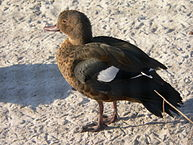
\includegraphics[width=4.3cm]{images/Ente}
    \caption{\small{Quelle: wikimedia}}
\end{wrapfigure}
Hier kommt nun viel Text. Hier kommt nun viel Text. Hier kommt nun viel Text. Hier kommt nun viel Text. Hier kommt nun viel Text. Hier kommt nun viel Text. Hier kommt nun viel Text. Hier kommt nun viel Text. Hier kommt nun viel Text. Hier kommt nun viel Text.  Hier kommt nun viel Text. Hier kommt nun viel Text. Hier kommt nun viel Text. Hier kommt nun viel Text. Hier kommt nun viel Text. Hier kommt nun viel Text. Hier kommt nun viel Text. Hier kommt nun viel Text. Hier kommt nun viel Text. Hier kommt nun viel Text. Hier kommt nun viel Text. Hier kommt nun viel Text. Hier kommt nun viel Text. Hier kommt nun viel Text. Hier kommt nun viel Text. Hier kommt nun viel Text. Hier kommt nun viel Text. Hier kommt nun viel Text. Hier kommt nun viel Text. Hier kommt nun viel Text. Hier kommt nun viel Text. Hier kommt nun viel Text. Hier kommt nun viel Text. Hier kommt nun viel Text. Hier kommt nun viel Text. Hier kommt nun viel Text. Hier kommt nun viel Text. Hier kommt nun viel Text. Hier kommt nun viel Text. Hier kommt nun viel Text.   Hier kommt nun viel Text.
\par\smallskip %Kleiner Absatz
Hier kommt nun viel Text. Hier kommt nun viel Text. Hier kommt nun viel Text. Hier kommt nun viel Text. Hier kommt nun viel Text. Hier kommt nun viel Text. Hier kommt nun viel Text. Hier kommt nun viel Text. Hier kommt nun viel Text. Hier kommt nun viel Text. Hier kommt nun viel Text. Hier kommt nun viel Text. Hier kommt nun viel Text.   Hier kommt nun viel Text. Hier kommt nun viel Text. Hier kommt nun viel Text. Hier kommt nun viel Text. Hier kommt nun viel Text. Hier kommt nun viel Text. Hier kommt nun viel Text. Hier kommt nun viel Text. Hier kommt nun viel Text. Hier kommt nun viel Text.   Hier kommt nun viel Text. Hier kommt nun viel Text. Hier kommt nun viel Text. Hier kommt nun viel Text. Hier kommt nun viel Text.   Hier kommt nun viel Text.
\par\bigskip %Großer Absatz

Damit die folgende Literaturliste angezeigt wird, müsst ihr eure Literatur in die bib.bib Datei eintragen und anschließend zunächst pdflatex ausführen, danach bibtex, danach wieder pdflatex.

\appendix
\section{Sample CSPs and Output}

\todo[inline]{Sample CSP mit Output}

\section{Commented Source Code}

\todo[inline]{Keine Ahnung ob wir das tun sollten... Vielleicht den entscheidenen Teil oder so?}

\bibliographystyle{plain}
\bibliography{bib}

\end{document}
